\begin{figure}[htbp]
\section*{ SCN2A}
\centering
\begin{subfigure}[b]{0.95\textwidth}
\centering
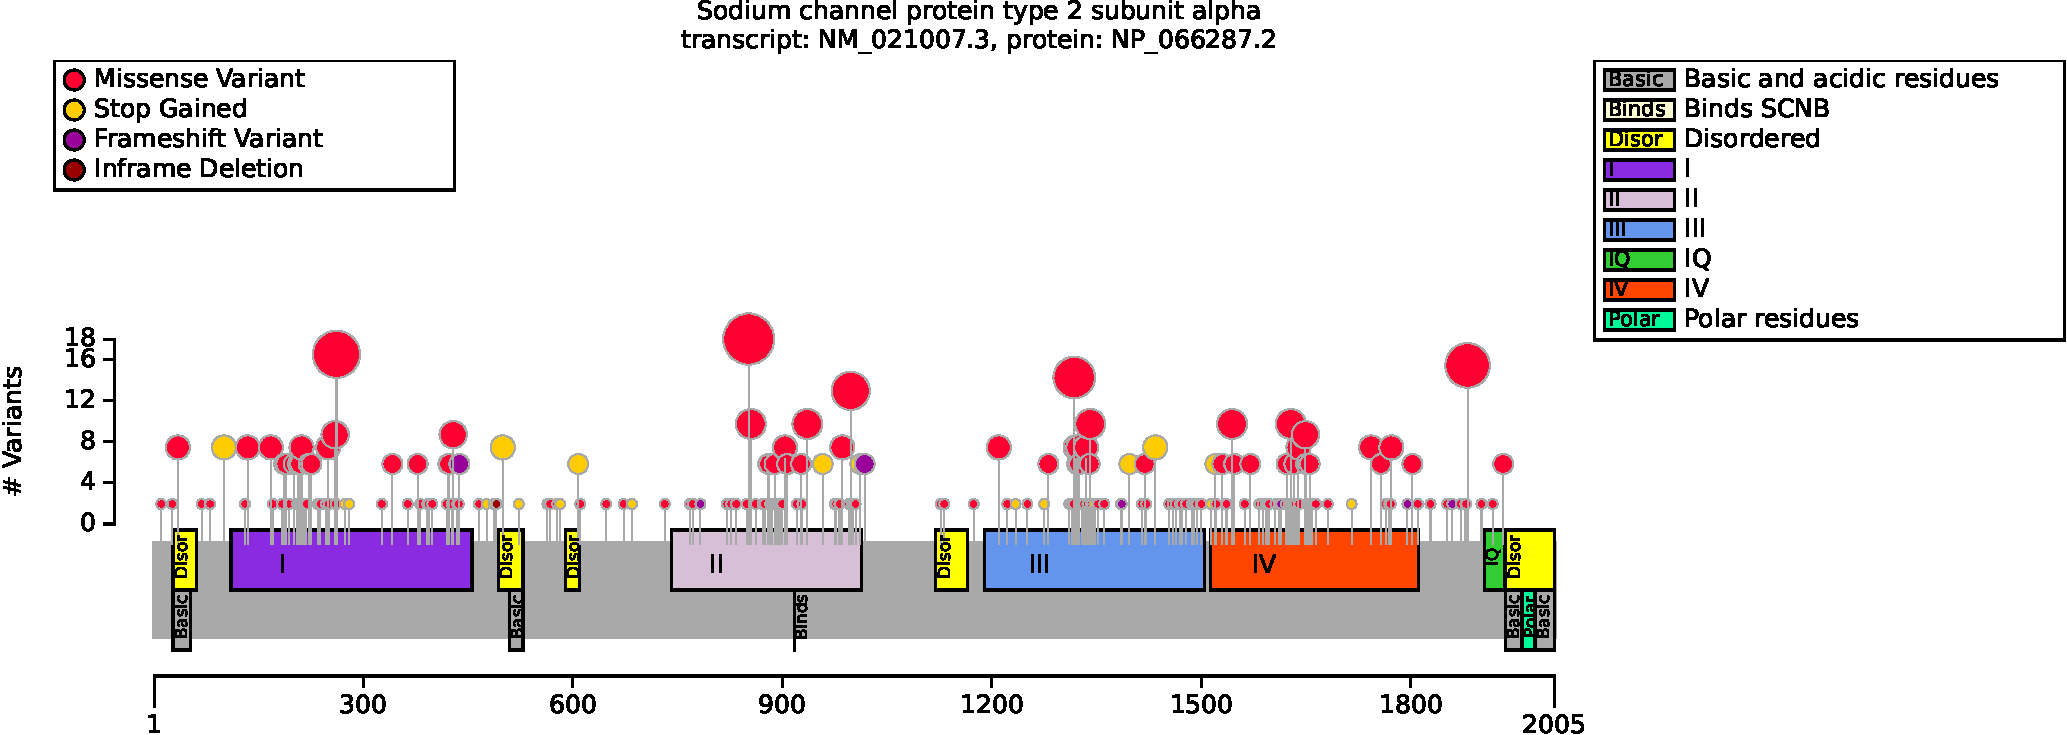
\includegraphics[width=\textwidth]{ img/SCN2A_protein_diagram.pdf} 
\captionsetup{justification=raggedright,singlelinecheck=false}
\caption{Distribution of variants in SCN2A}
\end{subfigure}

\vspace{2em}

\begin{subfigure}[b]{0.95\textwidth}
\centering
\resizebox{\textwidth}{!}{
\begin{tabular}{llllrr}
\toprule
HPO term & Missense & Other & p-value & adj. p-value\\
\midrule
Neurodevelopmental abnormality [HP:0012759] & 201/238 (84\%) & 45/45 (100\%) & 0.001 & 0.003\\
Motor seizure [HP:0020219] & 146/175 (83\%) & 6/31 (19\%) & $4.51\times 10^{-12}$ & $7.22\times 10^{-11}$\\
Seizure [HP:0001250] & 298/327 (91\%) & 28/53 (53\%) & $1.57\times 10^{-10}$ & $8.38\times 10^{-10}$\\
Autism [HP:0000717] & 59/146 (40\%) & 33/43 (77\%) & $2.69\times 10^{-5}$ & $8.61\times 10^{-5}$\\
Focal-onset seizure [HP:0007359] & 141/170 (83\%) & 8/33 (24\%) & $8.66\times 10^{-11}$ & $6.93\times 10^{-10}$\\
Generalized-onset seizure [HP:0002197] & 104/133 (78\%) & 6/31 (19\%) & $1.43\times 10^{-9}$ & $5.72\times 10^{-9}$\\
Intellectual disability [HP:0001249] & 144/198 (73\%) & 34/34 (100\%) & $9.39\times 10^{-5}$ & $2.50\times 10^{-4}$\\
\bottomrule
\end{tabular}
}
\captionsetup{justification=raggedright,singlelinecheck=false}
\caption{         Fisher Exact Test performed to compare HPO annotation frequency with respect to Missense and Other. Total of
        16 tests were performed. }
\end{subfigure}
\vspace{2em}
\begin{subfigure}[b]{0.95\textwidth}
\centering
\resizebox{\textwidth}{!}{
\begin{tabular}{llllrr}
\toprule
HPO term & I repeat & Other & p-value & adj. p-value\\
\midrule
Neurodevelopmental abnormality [HP:0012759] & 48/65 (74\%) & 198/218 (91\%) & 0.001 & 0.009\\
Intellectual disability [HP:0001249] & 21/42 (50\%) & 157/190 (83\%) & $2.59\times 10^{-5}$ & $4.15\times 10^{-4}$\\
\bottomrule
\end{tabular}
}
\captionsetup{justification=raggedright,singlelinecheck=false}
\caption{         Fisher Exact Test performed to compare HPO annotation frequency with respect to I repeat and Other. Total of
        16 tests were performed. }
\end{subfigure}
\vspace{2em}
\begin{subfigure}[b]{0.95\textwidth}
\centering
\resizebox{\textwidth}{!}{
\begin{tabular}{llllrr}
\toprule
Genotype (A) & Genotype (B) & total tests performed & significant results\\
\midrule
Arg853Gln & Other & 16 & 0\\
Exon 27 & Other & 16 & 0\\
\bottomrule
\end{tabular}
}
\captionsetup{justification=raggedright,singlelinecheck=false}
\caption{ Fisher Exact Test performed to compare HPO annotation frequency with respect to genotypes. }
\end{subfigure}

\vspace{2em}

\caption{ The cohort comprised 393 individuals (0 females, 0 males, 393 with unknown sex). A total of 289 HPO terms were used to annotate the cohort. Disease diagnoses: Developmental and epileptic encephalopathy 11 (OMIM:613721) (342 individuals), Seizures, benign familial infantile, 3 (OMIM:607745) (51 individuals). Similar genotype-phenotype correlations have been previously published \cite{PMID_31904126}. A total of 264 unique variant alleles were found in \textit{SCN2A} (transcript: \texttt{NM\_021007.3}, protein id: \texttt{NP\_066287.2}).}
\end{figure}
